\documentclass[12pt]{article}

\usepackage{amsmath, mathtools}
\usepackage{amsfonts}
\usepackage{amssymb}
\usepackage{graphicx}
\usepackage{colortbl}
\usepackage{xr}
\usepackage{hyperref}
\usepackage{longtable}
\usepackage{xfrac}
\usepackage{tabularx}
\usepackage{float}
\usepackage{siunitx}
\usepackage{booktabs}
\usepackage{caption}
\usepackage{pdflscape}
\usepackage{afterpage}
\usepackage[none]{hyphenat}
\usepackage[document]{ragged2e}
\usepackage[round]{natbib}

%\usepackage{refcheck}

\hypersetup{
    bookmarks=true,         % show bookmarks bar?
      colorlinks=true,       % false: boxed links; true: colored links
    linkcolor=red,          % color of internal links (change box color with linkbordercolor)
    citecolor=green,        % color of links to bibliography
    filecolor=magenta,      % color of file links
    urlcolor=cyan           % color of external links
}

%% Comments

\usepackage{color}

\newif\ifcomments\commentstrue %displays comments
%\newif\ifcomments\commentsfalse %so that comments do not display

\ifcomments
\newcommand{\authornote}[3]{\textcolor{#1}{[#3 ---#2]}}
\newcommand{\todo}[1]{\textcolor{red}{[TODO: #1]}}
\else
\newcommand{\authornote}[3]{}
\newcommand{\todo}[1]{}
\fi

\newcommand{\wss}[1]{\authornote{blue}{SS}{#1}} 
\newcommand{\plt}[1]{\authornote{magenta}{TPLT}{#1}} %For explanation of the template
\newcommand{\an}[1]{\authornote{cyan}{Author}{#1}}

%% Common Parts

\newcommand{\progname}{Mechatronics} % PUT YOUR PROGRAM NAME HERE
\newcommand{\authname}{Team \#20, Team Name
\\ Robert Zhu zhul49
\\ Zifan Meng mengz17
\\ Jiahui Chen chenj194
\\ Kelvin Huynh huynhk12
\\ Runze Zhu zhur25
\\ Mirza Nafi Hasan hasanm21} % AUTHOR NAMES                  

\usepackage{hyperref}
    \hypersetup{colorlinks=true, linkcolor=blue, citecolor=blue, filecolor=blue,
                urlcolor=blue, unicode=false}
    \urlstyle{same}
                                


% For easy change of table widths
\newcommand{\colZwidth}{1.0\textwidth}
\newcommand{\colAwidth}{0.13\textwidth}
\newcommand{\colBwidth}{0.82\textwidth}
\newcommand{\colCwidth}{0.1\textwidth}
\newcommand{\colDwidth}{0.05\textwidth}
\newcommand{\colEwidth}{0.8\textwidth}
\newcommand{\colFwidth}{0.17\textwidth}
\newcommand{\colGwidth}{0.5\textwidth}
\newcommand{\colHwidth}{0.28\textwidth}

% Used so that cross-references have a meaningful prefix
\newcounter{defnum} %Definition Number
\newcommand{\dthedefnum}{GD\thedefnum}
\newcommand{\dref}[1]{GD\ref{#1}}
\newcounter{datadefnum} %Datadefinition Number
\newcommand{\ddthedatadefnum}{DD\thedatadefnum}
\newcommand{\ddref}[1]{DD\ref{#1}}
\newcounter{theorynum} %Theory Number
\newcommand{\tthetheorynum}{T\thetheorynum}
\newcommand{\tref}[1]{T\ref{#1}}
\newcounter{tablenum} %Table Number
\newcommand{\tbthetablenum}{T\thetablenum}
\newcommand{\tbref}[1]{TB\ref{#1}}
\newcounter{assumpnum} %Assumption Number
\newcommand{\atheassumpnum}{P\theassumpnum}
\newcommand{\aref}[1]{A\ref{#1}}
\newcounter{goalnum} %Goal Number
\newcommand{\gthegoalnum}{P\thegoalnum}
\newcommand{\gsref}[1]{GS\ref{#1}}
\newcounter{instnum} %Instance Number
\newcommand{\itheinstnum}{IM\theinstnum}
\newcommand{\iref}[1]{IM\ref{#1}}
\newcounter{reqnum} %Requirement Number
\newcommand{\rthereqnum}{P\thereqnum}
\newcommand{\rref}[1]{R\ref{#1}}
\newcounter{nfrnum} %NFR Number
\newcommand{\rthenfrnum}{NFR\thenfrnum}
\newcommand{\nfrref}[1]{NFR\ref{#1}}
\newcounter{lcnum} %Likely change number
\newcommand{\lthelcnum}{LC\thelcnum}
\newcommand{\lcref}[1]{LC\ref{#1}}

\usepackage{fullpage}

\newcommand{\deftheory}[9][Not Applicable]
{
\newpage
\noindent \rule{\textwidth}{0.5mm}

\paragraph{RefName: } \textbf{#2} \phantomsection 
\label{#2}

\paragraph{Label:} #3

\noindent \rule{\textwidth}{0.5mm}

\paragraph{Equation:}

#4

\paragraph{Description:}

#5

\paragraph{Notes:}

#6

\paragraph{Source:}

#7

\paragraph{Ref.\ By:}

#8

\paragraph{Preconditions for \hyperref[#2]{#2}:}
\label{#2_precond}

#9

\paragraph{Derivation for \hyperref[#2]{#2}:}
\label{#2_deriv}

#1

\noindent \rule{\textwidth}{0.5mm}

}

\begin{document}

\title{Software Requirements Specification for \progname: ASL Translator} 
\author{\authname}
\date{\today}

\maketitle

~\newpage

\pagenumbering{roman}

\tableofcontents

~\newpage

\section*{Revision History}

\begin{tabularx}{\textwidth}{p{3cm}p{2cm}X}
\toprule {\bf Date} & {\bf Version} & {\bf Notes}\\
\midrule
Date 1 & 1.0 & Notes\\
Date 2 & 1.1 & Notes\\
\bottomrule
\end{tabularx}

~\newpage

\section{Reference Material}

\subsection{Terms, Abbreviations, and Acronyms}

\renewcommand{\arraystretch}{1.2}
\noindent \begin{tabularx}{\textwidth}{p{0.3\linewidth}|X}
\toprule
\textbf{Term, Abbreviation, or Acronym} & \textbf{Description}\\
\midrule
A
& Shorthand for Assumption\\
\hline
ASL
& Shorthand for American Sign Language. It is a form of sign language primarily used in the US and in parts of Canada\\
\hline
CFR
& Shorthand for Camera Functional Requirement\\
\hline
CMC
& Shorthand for carpometacarpal. This is the joint that connects your thumb to the rest of your hand\\
\hline
DIP
& Shorthand for distal interphalangeal. This is the joint on your finger just before where your fingernail is\\
\hline
IP
& Shorthand for interphalangeal. This is the joint just before where your fingernail on the thumb is situated\\
\hline
MCP
& Shorthand for metacarpophalangeal. This is the joint situated roughly where your knuckles are\\
\hline
ML
& Shorthand for Machine Learning\\
\hline
MLFR
& Shorthand for Machine Learning Functional Requirement\\
\hline
NFR
& Shorthand for Non-Functional Requirement\\
\hline
OpenCV (shortened to CV)
& A library of programming tools that enable real-time computer vision. OpenCV provides a basic infrastructure 
for computer applications that require the use of cameras\\
\hline
PIP 
& Shorthand for proximal interphalangeal. This is the next joint up your finger from where the knuckles are\\
\hline
TensorFlow
& An open-source framework developed by Google, which enables machine learning, deep learning, and other 
statistical and predictive analytics\\
\bottomrule
\end{tabularx}

\newpage

\pagenumbering{arabic}

\section{Introduction}
\subsection{Purpose of the Project}
\indent The purpose of our project is to create a device that will translate sign language gestures into their corresponding words or phrases. This will require
the creation and development of a computer vision system alongside a machine learning model that will be used to recognize the hand motions, as well as a 
Raspberry Pi that will speak the word or phrase. The user will perform the sign language motion that will be captured by our computer vision system through
a camera, and processed by our machine learning model and spoken through our Raspberry Pi.

\subsection{Scope} 
\subsubsection{In-Scope} \label{sec_inScope}
\indent The goals for our project are listed in the following table. The primary goals for our project include
\begin{itemize}
    \item Accurate hand motion recognition: Tracking and recognition of the user\textquotesingle s hands
    \item Real-time translation: Recognition and translation of user\textquotesingle s hand gestures with minimal delay
\end{itemize}

\renewcommand{\arraystretch}{1.2}
\noindent \begin{tabularx}{\textwidth}{p{0.2\linewidth}|p{0.72\linewidth}}
\toprule
\textbf{Goals} & \textbf{Desciption}\\
\midrule
Reliable and Accurate Translations
& The Sign Language Translator requires extensive training on the sensors to capture precise hand motion
and ignore any human error on the user\textquotesingle s part. The processing unit should be able to identify each letter 
within the American Sign Language using the data collected and transmit dialogue accurately to the user\textquotesingle s 
request.\\
\hline
Real Time Translations
& User\textquotesingle s should never be required to wait an extensive period of time for the device to process their hand 
motion and provide a translation. The Sign Language Translator should simulate a real time conversation between
regular people to deliver a seamless transition for other parties during presentations or social interactions.\\
\hline
Ease of Use
& The user experience is crucial for a communication device. The Sign Language Translator should require minimal 
time and effort to set up. Once set up, the device should not require much maintenance or updates. Most importantly,
the device should not hinder the user\textquotesingle s ability to perform the gestures and hand motions of sign language.\\
\hline
Affordability
& The Sign Language Translator should be affordable for the end users as to reduce the need of requiring an actual 
translator to accompany the user during their tasks. The device should remain functional whenever it is required to 
be used, and the hardware components of the device should be simple and cost-effective.\\
\hline
Customizable to User
& As with language, different people might have a certain way of pronouncing a phrase or word and likewise the same 
could be said with Sign Language with slightly different gestures. The device should be able to adapt to the user and 
recognize the unique motions instead of forcing the user to slow down for the device.\\
\bottomrule
\end{tabularx}

\subsubsection{Out-of-Scope}
\indent The stretch goals for our project are listed in the following table. These goals are out-of-scope for our 
project. They may or may not be achieved depending on our progress and time remaining in the academic year.

\renewcommand{\arraystretch}{1.2}
\noindent \begin{tabularx}{\textwidth}{p{0.2\linewidth}|p{0.72\linewidth}}
\toprule
\textbf{Stretch Goals} & \textbf{Desciption}\\
\midrule
Portable
& The final device, while requiring OpenCV to scan and process hand motion, should become more portable and lightweight 
for the user to move around, so as to not interfere with the user’s regular activities. The translator text to speech 
should become an application on all phone brands as for any user with the required equipment to be able to begin using.\\
\hline
Expanding to Different Languages
& As a universal sign language does not exist at the moment, there exists deaf/mute individuals who use another form of 
sign language other than the American Sign language. These include the British, Australian and New Zealand Sign Language (BANZSL),
the Chinese Sign Language (CSL), Arabic Sign language, and much more. The device should be able to understand and translate these 
new hand motions and generate a translation in their native language for this product to be used on a global scale.\\
\hline
Sign Language Education
& The final device should be able to recognize the different hand motions and gestures of sign language in order to accurately
translate them. This would make the device an excellent educational tool for those looking to learn sign language. The device 
could provide feedback and tell users how to improve their gestures using it’s accurate hand tracking to help teach those unfamiliar 
with sign language.\\
\hline
Non-real Time Translations
& The final product should be able to extract and recognize hand gestures from photos or videos uploaded by the users. 
In this case, if the users find online photos or videos related to sign language, they can upload them to application/software
to acquire text-based translation. This could help the users learn sign language from online sources.\\
\bottomrule
\end{tabularx}

\subsection{Usual Operations}

\subsection{Users and Stakeholders}

\section{Project Constraints}
\subsection{Constraints}
\indent The project is constrained by the following:
\begin{itemize}
  \item Translate a subset of the American Sign Language (ASL)
  \begin{itemize}
    \item Training a machine learning model to encompass the entire ASL would be very time-inefficient for the time constraint of the project
  \end{itemize}
  \item The project expenses cannot exceed \$750 CAD
  \begin{itemize}
    \item Additionally the project cannot be an off-the-shelf solution and be cost-efficient to attain our goal of affordability
  \end{itemize}
  \item The project must be completed during the course of the academic year
  \begin{itemize}
    \item This serves as a time constraint for the project and is also a requirement set by the course
  \end{itemize}
\end{itemize}

\subsection{Assumptions}

\section{Context Diagrams}

\begin{figure}[H] 
\centering
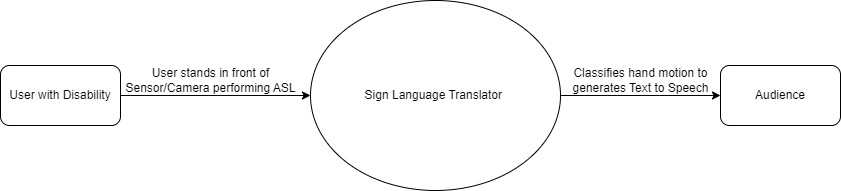
\includegraphics[width=1\textwidth]{Context Diagram} 
\caption{Context Diagram} 
\label{Fig.Context_Diagram} 
\end{figure}

\section{Functional Decomposition}
\subsection{Data Flow Model}

\subsection{Monitor and Controlled Variables}

\section{Functional Requirements}
\subsection{Camera Functional Requirements}

\renewcommand{\arraystretch}{1.2}
\noindent \begin{tabularx}{\textwidth}{p{0.12\linewidth}|p{0.4\linewidth}|p{0.4\linewidth}}
\toprule
\textbf{Identifier} & \textbf{Requirement} & \textbf{Rationale}\\
\midrule
CFR1 
& User hand gestures should be recognized and converted into input for the system 
& This is the primary and only way that the end user engages with the system. This is to ensure that 
their signing is picked up by the camera within a certain degree of accuracy\\
\hline
CFR2
& The camera must be able to relay its vision back to the program
& This enables validation and testing on the development end. In addition to understanding what needs 
to be corrected to ensure accurate user input\\
\bottomrule
\end{tabularx}

\subsection{Machine Learning Functional Requirements}

\renewcommand{\arraystretch}{1.2}
\noindent \begin{tabularx}{\textwidth}{p{0.12\linewidth}|p{0.4\linewidth}|p{0.4\linewidth}}
\toprule
\textbf{Identifier} & \textbf{Requirement} & \textbf{Rationale}\\
\midrule
MLFR1 
& The program should be able to recognize user hand joints
& This enables the ML model to compare and match user hand gestures to ASL\\
\hline
MLFR2 
& The program should output the x, y, and z coordinates of each joint relative to the camera
& This will enable system calibration and aid in enhancing predictive accuracy as the training 
data set will be primarily static images in contrast to the dynamic input from the end product\\
\hline
MLFR3 
& The program should recognize up to two hands in the input
& The complexity of sign language calls for two hands to enable effective communication. 
Tracking one hand should also be considered as there are words in sign language that require the 
use of a single hand\\
\hline
MLFR4 
& The program should be able to process data in real-time
& The translator should relay the relevant translation within a reasonable amount of time to ensure 
conversation fluidity\\
\hline
MLFR5 
& The program must be able to calibrate the camera
& This is to ensure that the image being processed is undistorted and recognizable to the program 
to prevent inaccuracies and incorrect output from the ML model\\
\hline
MLFR6 
& The program should be calibrated to match the speed of the signer
& The translator should be able to keep up with the user or the likelihood of a mistranslation will increase\\
\hline
MLFR7 
& The ML model should be easily trainable
& This is how the ML model should learn sign language to use in processing. Making it easily trainable should 
enable expandability as well. In addition, this will enable the program to adapt to users\textquotesingle \ specific signing 
habits and allow for manual correction for the future\\
\bottomrule
\end{tabularx}

\section{Functional Requirement Change Likelihood}
\subsection{Camera Functional Requirements}

\renewcommand{\arraystretch}{1.2}
\noindent \begin{tabularx}{\textwidth}{p{0.12\linewidth}|p{0.15\linewidth}|p{0.3\linewidth}|p{0.3\linewidth}}
\toprule
\textbf{Identifier} & \textbf{Likelihood of Change} & \textbf{Rationale} & \textbf{What May Be Changed}\\
\midrule
CFR1 
& Unlikely
& Input component of the system
& Input may be changed to sensor instead of a camera\\
\hline
CFR2
& Very unlikely
& Enables testing and validation for the system
& N/A\\
\bottomrule
\end{tabularx}

\subsection{Machine Learning Functional Requirements}

\renewcommand{\arraystretch}{1.2}
\noindent \begin{tabularx}{\textwidth}{p{0.12\linewidth}|p{0.15\linewidth}|p{0.3\linewidth}|p{0.3\linewidth}}
\toprule
\textbf{Identifier} & \textbf{Likelihood of Change} & \textbf{Rationale} & \textbf{What May Be Changed}\\
\midrule
MLFR1 
& Very unlikely
& Key processing component of the system
& N/A\\
\hline
MLFR2 
& Very unlikely
& Enables testing and validation for the system
& N/A\\
\hline
MLFR3 
& Unlikely
& Subject to time constraint. ML model accuracy may be sub-par for two hand input
& Tracking might only be possible with one hand\\
\hline
MLFR4 
& Unlikely
& Subject to time constraint. Refer to \ref{sec_inScope}
& Data processing in real-time may be difficult and delays might have to be used to ensure translation is as accurate is possible\\
\hline
MLFR5 
& Very unlikely
& Key processing component of the system
& N/A\\
\hline
MLFR6 
& Unlikely
& Key implementation aspect. Refer to \ref{sec_inScope}
& Dependent on the processing speed of the program. The speed at which a user can input sign language might be reduced consequently\\
\hline
MLFR7 
& Likely
& Key implementation aspect. But expandability of the program is subject to time constraint and memory required
& The ML model may only accommodate a subset of ASL for the sake of time constraint and space saving\\
\bottomrule
\end{tabularx}

\section{Non-functional Requirements}
\subsection{Accuracy Requirement}

\subsection{Useability Requirement}

\subsection{Portability Requirement}

\section{References}

\section{Appendix}
\subsection{Reflection}

\end{document}
